\chapter{Test}
\section{Test site}
The test site consist of the obstacles stated in table \ref{tab:obstacles}. Pictures of the test site can be found in chapter \ref{ch:testSite}.

\begin{table} [h]
    \centering
    \begin{tabu} to 1\textwidth { | X[c] | X[c] | X[c] | }
     \hline
     Obstacles & \multicolumn{2}{c|}{Size} \\
     \hline
     Football table & Length 145cm & Width 75cm \\
     \hline
     Bucket & Diameter 35cm & \\
    \hline
     Bench & Length 200cm & Width 40cm \\
     \hline
     Carpet & Length 200cm & Width 115cm \\
     \hline
     Small pot & Length 35cm & Width 35cm \\
     \hline
     Big pot & Length 95cm & Width 40cm \\
     \hline
     Upper staircase  & Length 180cm & Width 115cm \\
     \hline
     Lower staircase  & Length 600cm & Depth 18cm \\
     \hline
    \end{tabu}
    \caption{Table of the sizes of all obstacles from the test site}
    \label{tab:obstacles}
\end{table}
\begin{figure}[h]
    \centering
    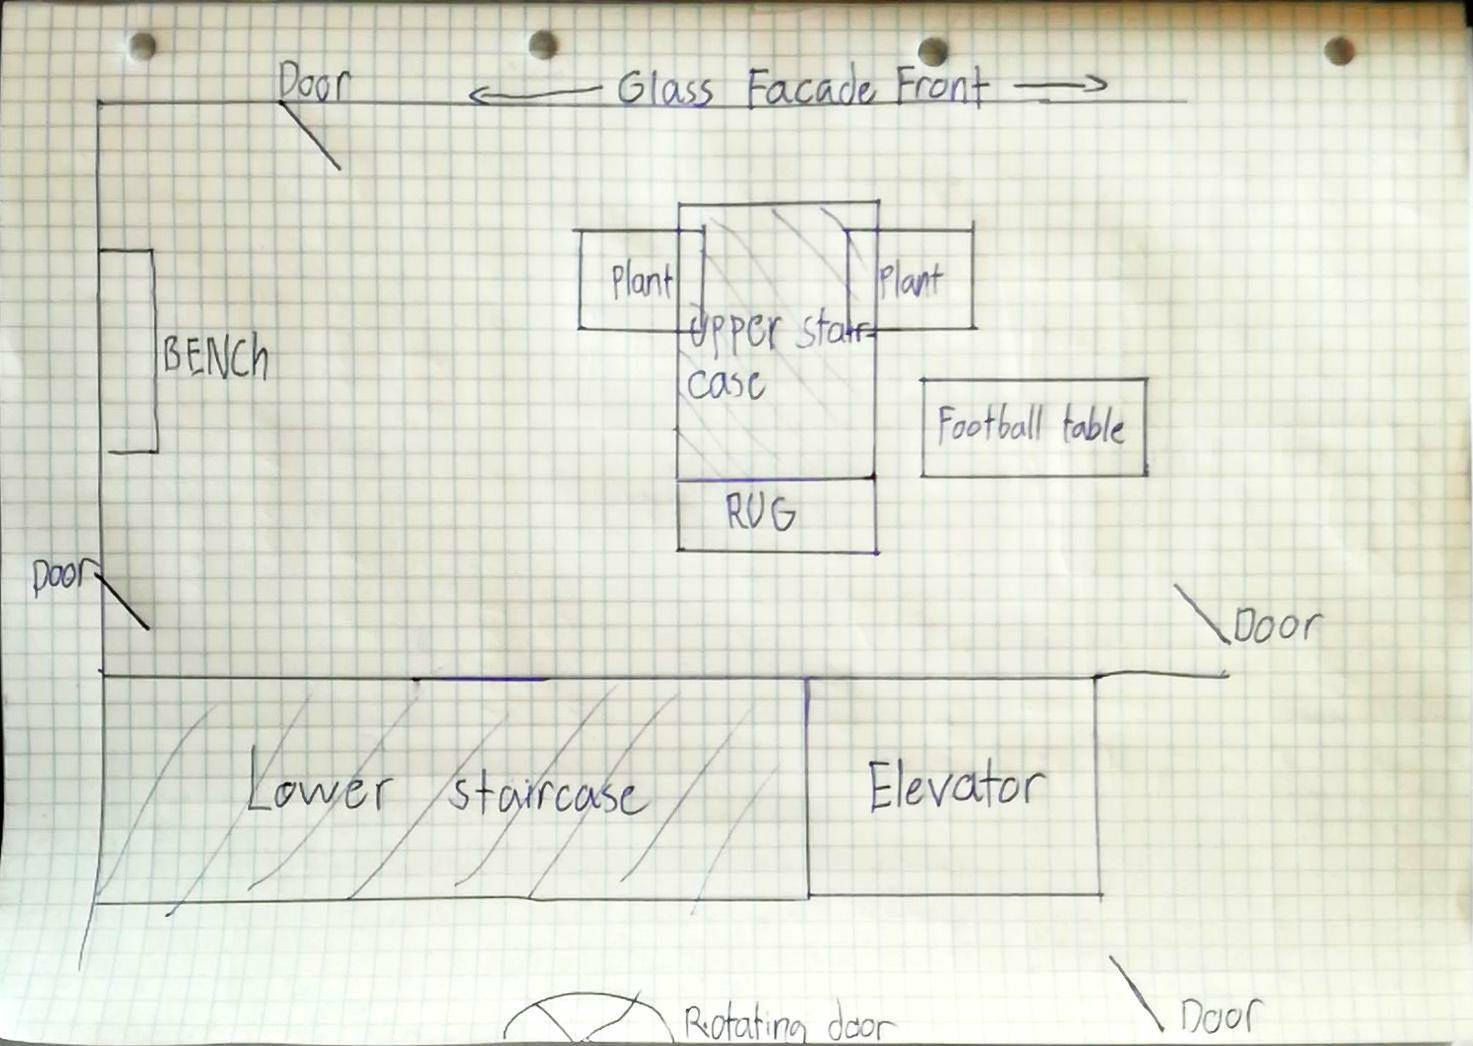
\includegraphics[width=\textwidth]{figures/layout.jpg}
    \caption{Test site layout} 
    \label{fig:layout} 
\end{figure}
%
% Test 1
%

\section{Test 1}
Purpose of test 1: Communication between the robot, ROS and the computer.\\
The motor control of the turlebot will be testet. First the host computer gets the following commands:\\
1. \texttt{roscore}\\ 
2. \texttt{roslaunch\_bringup minimal.launch}\\
Then the user computer gets the following commands:\\ 
1. \texttt{roslaunch turtlebot\_teleop keyboard\_teleop.launch}\\
The user computer should now be able to control the turtlebot. 

\subsection{1st run}
What was done:\\ 
The Robots velocity was set to 0.2 m/s. The robot was steered with \texttt{Roslaunch turtlebot\_teleop keyboard\_teleop.launch} from the computer where the keyboard was used to control the robot.\\
The robot would then move accordingly to the keys 'J', 'L', 'I', ',' and 'K'.
\begin{itemize}
    \item J for left.
    \item L for right.
    \item I for forward.
    \item , for backwards.
    \item K for stopping.
\end{itemize}
What happened:\\
The turtlebot had no problems being controlled manually. The connection between computer and ROS MASTER was established and working well. When moving on the carpet, the velocity fell and first after second try the turtlebot would push forward, and would not get stuck.\\
Since it was controlled manually, it could not measure itself towards the obstacles, therefore it had no problem running beneath the staircase and under the football table. 

\subsection{2nd run}
What was done:\\
The turtlebot velocity was set to 0.8 m/s and steered as mentioned in the 1st run.\\
What happened:\\
The turtlebot  had to be stopped a couple of times due to the high speed. When using the \texttt{teleop} package, the turtlebot experienced some delay, and when turning and moving forward it was a problem to stop.

\subsection{3rd run}
What was done: \\
In this test the velocity was set to 0.4 m/s and steered as mentioned in the 1st run. There was also an attempt to see if the cliff sensor worked in manual mode.\\
What happened:\\
The turtlebot had no problems being controlled, but the cliff sensor did not work since the host computer did not run \textit{g\_mapping} node. 



%
% Test 2
%

\section{Test 2}
Purpose of test 2: Detecting Obstacles.\\ 
First the host computer gets the commands:\\
1. \texttt{roscore}\\
2. \texttt{roslaunch\_bringup minimal.launch}\\
3. \texttt{roslaunch turtlebot\_navigation gmapping\_demo.launch}\\
On the user computer the commands is written in two seperate terminals:\\
1. \texttt{roslaunch turtlebot\_teleop keyboard\_teleop}\\
2. \texttt{roslaunch turtlebot\_rviz\_launchers view\_navigation.launch.}\\
A window will appear with robot vision. The terminal with the \textit{teleop package} keyboard can be used to move the turtlebot. The window will make a map with obstacles.
It will be tested with different speeds to see the better result.

\subsection{1st run}
What was done:\\
The turtlebot was controlled by the user computer manually, while it was mapping and creating a 2D map in Rviz. The turtlebot had a speed of 0.4 m/s. The turtlebot had to avoid obstacles and drive over different terrain, such as a carpet.\\
What happened:\\
The turtlebot had no problems being controlled manually and it detected the obstacles as expected while mapping. The turtlebot also had no problems driving over the carpet.

\subsection{2nd run}
What was done:\\
The speed was changed to 0.8 m/s and steered as mentioned in the 1st run.\\
What happened:\\
The turtlebot had difficulties being controlled manually and the mapping in Rviz could not keep up with the turtlebot's movements. The turtlebot could, with this speed, easier drive over the carpet than with the slower speed.

\subsection{3rd run}
What was done:\\
The speed was changed to 0.2 m/s and steered as mentioned in the 1st run.\\
What happened:\\
Because of the slower speed in 3rd run, Rviz had a chance to keep up with the turtlebot's mapping, which resulted in the map being more detailed compared to 2nd run. The robot had difficulties driving over carpet, but succeeded after trying two times.

%
% Test 3
%

\section{Test 3}
Purpose of test 3: Path-planning, the movement of base autonomously. 
1. \texttt{roscore}\\
2. \texttt{roslaunch\_bringup minimal.launch}\\
3. \texttt{roslaunch turtlebot\_navigation gmapping\_demo.launch}\\
On the user computer the commands is written in the terminal:\\
1. \texttt{roslaunch turtlebot\_rviz\_launchers view\_navigation.launch.}\\
A window will appear with robot vision, using nav 2D goal to make a path for the turtlebot.

\subsection{1st run}
What was done:\\
The software capability to autonomously navigate the robot around objects towards a goal was tested.\\
What happened:\\
Max\_vel\_x was set as default.\\
It was able to map and detect  the soccer table, which it managed to drive under on its route towards its goal. It also detected the carpet, which it managed to pass over, but upon detecting the difference in surface friction on top of the carpet, it stopped momentarily, before it continued on its path.\\
The test was stopped, since a lot of people was passing through and the software had trouble managing so many moving obstacles around its sensor.

\subsection{2nd run}
What was done:\\
Max\_vel\_x parameter was changed to 0.2, to see if the robot reacted differently with a lower velocity.\\
What happened:\\
With the low velocity, the robots mapping process was more detailed. Which resulted in the sensors observed the obstacles and avoided accordingly.

\subsection{3rd run}
What was done:\\
Max\_vel\_x parameter was changed to 0.005, to see if the robot reacted differently with such a low velocity.\\
What happened:\\
The test failed due to the velocity setting was too low.

%
% Test 4
%

\section{Test 4} 
What is the purpose of test 4:\\
Testing out frontier exploration will combine test 1, 2 and 3. Detecting Obstacles.\\ 
The host computer got the commands:\\
1.\texttt{roscore} 
2.\texttt{roslaunch\_bringup minimal.launch}\\
3.\texttt{roslaunch turtlebot\_navigation gmapping\_demo.launch}\\
The user computer was given the commands in two different terminals:\\
1.\texttt{roslaunch turtlebot\_rviz\_launchers view\_navigation.launch}\\
2.\texttt{roslaunch turtlebot\_samples exploration.launch}\\
Here it should be possible to make a polygon area in Rviz by using publishing points, that the robot will explore.

\subsection{1st run}
What was done:\\
A unknown environment was set up.\\ 
The group then entered a polygon with the publish points in Rviz, to make the robot explore that environment, with the speed at a default setting at 0.55.\\
What happened:
The turtlebot 
\\


\subsection{2nd run}
What was done:\\
The robot was again set to explore a new area. The velocity was set to 0.2.\\
In this test the group wanted to see whether the cliff sensor worked.\\
What happened:\\
In this test, the navigation failed. There was a lot of different people that kept on passing the sensor. We observed that the robot made a static wall in the map due to all the passing people, and it would not drive further.\\
The group pinpointed a location for the robot to start driving, which was the lower staircase. The robot would then drive until the infrared sensor underneath its chassis could sense a drop, then it would redo this until it was parallel with the staircase.

\subsection{3rd run}
What was done:\\
The robot was again set to explore a new area. The velocity was set to 0.8.\\
What happened:
In this run with 0.8, the turtlebot had difficulty in making a route to follow. It failed to explore any part of the selected area, it went into recovery mode and stopped working.

%
% Test 5
%

\section{Test 5}
What is the purpose of test 5: \\
Redoing test 4, but with extra weight.

\subsection{1st run}
What was done:havent done yet
\\
What happened:havent done yet

\subsection{2nd run}
What was done:havent done yet
\\
What happened:havent done yet

\subsection{3rd run}
What was done:havent done yet
\\
What happened:havent done yet



